\documentclass[10pt, xcolor=dvipsnames]{beamer}
%\documentclass[10pt, xcolor=dvipsnames,notes=only]{beamer}
%\mode<presentation>
%{
\usetheme{Goettingen}
%\setbeamercovered{transparent}
%} 
\usefonttheme{professionalfonts}
%\usecolortheme{beaver}

\usepackage{setspace}
\usepackage[english]{babel}
\usepackage[latin1]{inputenc}
\usepackage{times}
\usepackage[T1]{fontenc}
\usepackage{color}
\usepackage{graphicx}
\usepackage{amssymb}
\usepackage{amsthm}
\usepackage{bm}
\usepackage{rotating}
\usepackage{ccaption}
\usepackage{booktabs}
\usepackage{lscape}
\usepackage{colortbl}
\usepackage{arydshln}
\usepackage{tabularx}
\usepackage{graphics}
\usepackage{epstopdf}

\setbeamertemplate{navigation symbols}{}
\setbeamertemplate{items}[balls]

\newenvironment{changemargin}[2]{%
  \begin{list}{}{%
    \setlength{\topsep}{0pt}%
    \setlength{\leftmargin}{#1}%
    \setlength{\rightmargin}{#2}%
    \setlength{\listparindent}{\parindent}%
    \setlength{\itemindent}{\parindent}%
    \setlength{\parsep}{\parskip}%
  }%
  \item[]}{\end{list}}

\setbeamercolor{block title}{fg=white, bg=teal}
\setbeamercolor{block body}{bg=teal!25}

\author[]{Chad Jones and Dietrich Vollrath}
\institute[Intro Growth]{Introduction to Economic Growth}
\date[]{}


\title[Romer]{The Romer Model of Growth}

\begin{document}
\maketitle

\section{Setup}
\begin{frame}{Productivity growth}
Productivity is central to GDP per capita in the Solow:
\begin{itemize}
	\item The growth rate, $g_A$, determines the long-run growth rate
	\item The level of productivity, $A_0$, is important for level of GDP per capita
\end{itemize}
Understanding what drives productivity growth is thus central to understanding economic growth
\end{frame}

\begin{frame}{Romer's model of growth}
We want a model of growth that:
\begin{itemize}
	\item Has all the elements of the Solow model
	\item Is specific about what $A$ means in that model
	\item Explains the dynamics of $A$ and $g_A$
	\item Explains why $g_A$ is constant along a BGP
	\item Requires effort to create the new ideas that drive $A$ and $g_A$
	\item Explains the choice involved in making that effort
\end{itemize}
\end{frame}

\begin{frame}{The Solow part}
Much of the model starts with familiar items. Production is
\begin{equation}
	Y_t = K_t^{\alpha}(A_t L_{Yt})^{1-\alpha} \label{EQ_final_romer}
\end{equation}
where $L_{Yt}$ are workers employed in producing goods and services. $L_{Rt}$ are people engaged in R\&D producing ideas, and
\begin{equation}
	L_t = L_{Yt} + L_{Rt}.
\end{equation}
denoting the ratio of R\&D workers as
\begin{equation}
	s_R = \frac{L_{Rt}}{L_t}.
\end{equation}
\end{frame}

\begin{frame}{The Solow part}
Standard parts:
\begin{itemize}
	\item Capital accumulates in the same way as in the Solow (depends on $K/AL$)
	\item Population growth is the same as in the Solow (exogenous at $g_L$)
\end{itemize}
Assuming that $g_A$ ends up constant (which we'll see) then economy ends up at steady state with a constant $K/AL$ ratio as usual.
\end{frame}

\section{Idea Accumulation}
\begin{frame}{Adding to ideas}
The relevant part of this Romer model is the accumulation of ideas. We start with pure mechanics.
\begin{equation}
	dA = \theta L_{Rt}^{\lambda} A_t^{\phi}. \label{EQ_dotA}
\end{equation}
The change in ideas (= productivity), $dA$, depends on
\begin{itemize}
	\item $\theta$. A parameter that governs how fast ideas accumulate
	\item $L_{Rt}$, the number of R\&D workers. More researchers, more ideas are found
	\item $A_t$, the existing stock of ideas. This could make new ideas easier or harder to find.
\end{itemize}
\end{frame}

\begin{frame}{Adding to ideas}
Same equation:
\begin{equation}
	dA = \theta L_{Rt}^{\lambda} A_t^{\phi}. \label{EQ_dotA}
\end{equation}
Two interesting parmeters. 
\begin{itemize}
	\item $0 < \lambda < 1$ measures how sensitive $dA$ is to $L_{Rt}$.
	\item If $\lambda$ is close to zero, then researchers ``crowd'' each other
	\item $-\infty < \phi < 1$ measure the effect of productivity on idea accumulation
	\item We'll see why $\phi < 1$ is crucial to stable outcomes
	\item If $0 \phi < 1$ higher prod makes new ideas easier (e.g. AI)
	\item If $\phi < 0$ higher prod makes new ideas harder (e.g. calculus is harder than the wheel)
\end{itemize}
\end{frame}

\begin{frame}{Adding to ideas}
Same equation:
\begin{equation}
	dA = \theta L_{Rt}^{\lambda} A_t^{\phi}. \label{EQ_dotA}
\end{equation}
Two interesting parmeters. 
\begin{itemize}
	\item $0 < \lambda < 1$ measures how sensitive $dA$ is to $L_{Rt}$.
	\item If $\lambda$ is close to zero, then researchers ``crowd'' each other
	\item $-\infty < \phi < 1$ measure the effect of productivity on idea accumulation
	\item We'll see why $\phi < 1$ is crucial to stable outcomes
	\item If $0 \phi < 1$ higher prod makes new ideas easier (e.g. AI)
	\item If $\phi < 0$ higher prod makes new ideas harder (e.g. calculus is harder than the wheel)
\end{itemize}
\end{frame}

\section{Dynamics}
\begin{frame}{Growth rate of ideas}
Divide both sides by $A$
\begin{equation}
	g_A = \frac{dA}{A_t} = \theta s_R^{\lambda} \frac{L_t^{\lambda}}{A_t^{1-\phi}}. \label{EQ_gA}
\end{equation}
The growth rate, $g_A$, depends on a ratio 
\begin{itemize}
	\item $L_t^{\lambda}/A_t^{1-\phi}$ is ``researcher per idea'' we employ
	\item $g_A$ is higher the bigger is this ratio
	\item Like capital growth, productivity growth depends negatively on productivity level
	\item Analyze dynamics via how $g_A$ responds to the ratio
\end{itemize}
\end{frame}

\begin{frame}{Tricky dynamics}
Given this:
\begin{equation}
	g_A = \theta s_R^{\lambda} \frac{L_t^{\lambda}}{A_t^{1-\phi}}. \label{EQ_gA}
\end{equation}
We want to graph the growth rate of both parts of the ratio:
\begin{itemize}
	\item Numerator growth rate is $\lambda g_L$. Given.
	\item Denominator growth rate is $(1-\phi)g_A$. Endogenous to ratio.
\end{itemize}
Like with $K/AL$, we'll plot the growth rate of numerator and denominator against the ratio
\end{frame}

\begin{frame}{Dynamics of productivity}
Patents Issued in the United States, by Country of Origin
\begin{center}
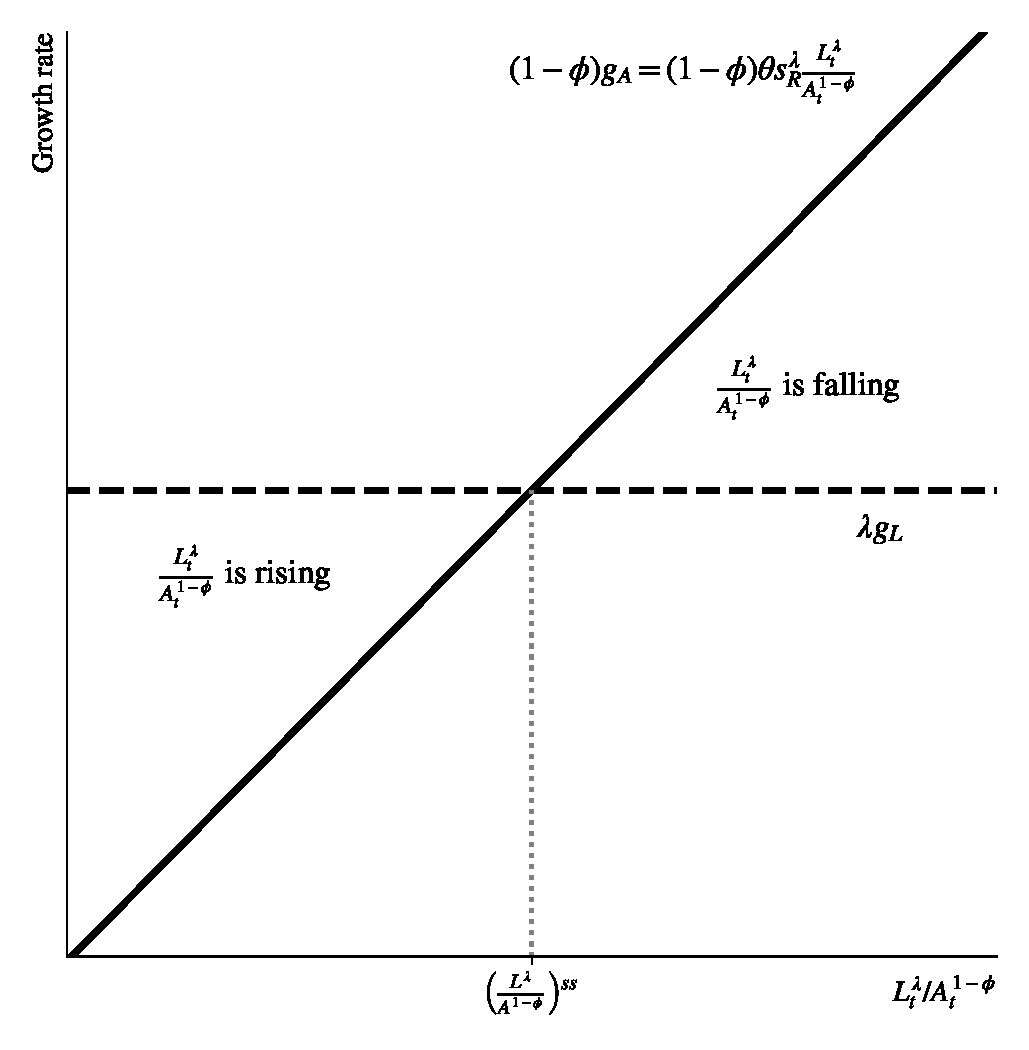
\includegraphics[height = 3in]{../Figures/fig-ch5-fig1.eps}
\end{center}
\end{frame}

\begin{frame}{Steady state}
No matter the initial ratio $L_0^{\lambda}/A_0^{1-\phi}$ the dynamics
\begin{itemize}
	\item Push the ratio towards a steady state where curves cross
	\item This happens because $g_A$ rises with ratio, but $g_L$ stays constant
	\item At that steady state $(1-\phi)g_A = \lambda g_L$
	\item Like with capital, the growth rate of the endogenous thing depends on the growth rate of the exogenous thing
\end{itemize}
\begin{block}{Long-run growth rate}
The long-run growth rate of productivity is
\begin{equation}
	g_A^{ss} = \frac{\lambda}{1-\phi}g_L
\end{equation}
\end{block}
\end{frame}

\begin{frame}{Long-run growth}
We just saw given our dynamics for ideas that
\begin{equation}
	g_A^{ss} = \frac{\lambda}{1-\phi}g_L
\end{equation}
The growth rate of productivity depends on the \textit{growth rate} of population. This is the non-rivalry of ideas eliminating the dilution of population growth (like on capital).

\vspace{.25in}\noindent Note what does \textit{not} influence the growth rate:
\begin{itemize}
	\item R\&D intensity, $s_R$
	\item The size of the labor force, $L$
	\item The level of GDP per capita
\end{itemize}
\end{frame}

\begin{frame}{Shocks and responses}
Like with the Solow we can investigate shocks to parameters. What is commit more resources to R\&D? 
\begin{itemize}
	\item Specifically, what if $s_R$ goes up?
	\item In the long-run, we know that the growth rate $g_A$ won't be different
	\item But in the short-run, that will raise the number of R\&D workers, raising $g_A$
	\item How do the dynamics explain the return to the long-run result?
	\item What happens to the level of productivity in response?
\end{itemize}
\end{frame}

\begin{frame}{Dynamics of $g_A$}
The Dynamics of an Increase in $s_R$
\begin{center}
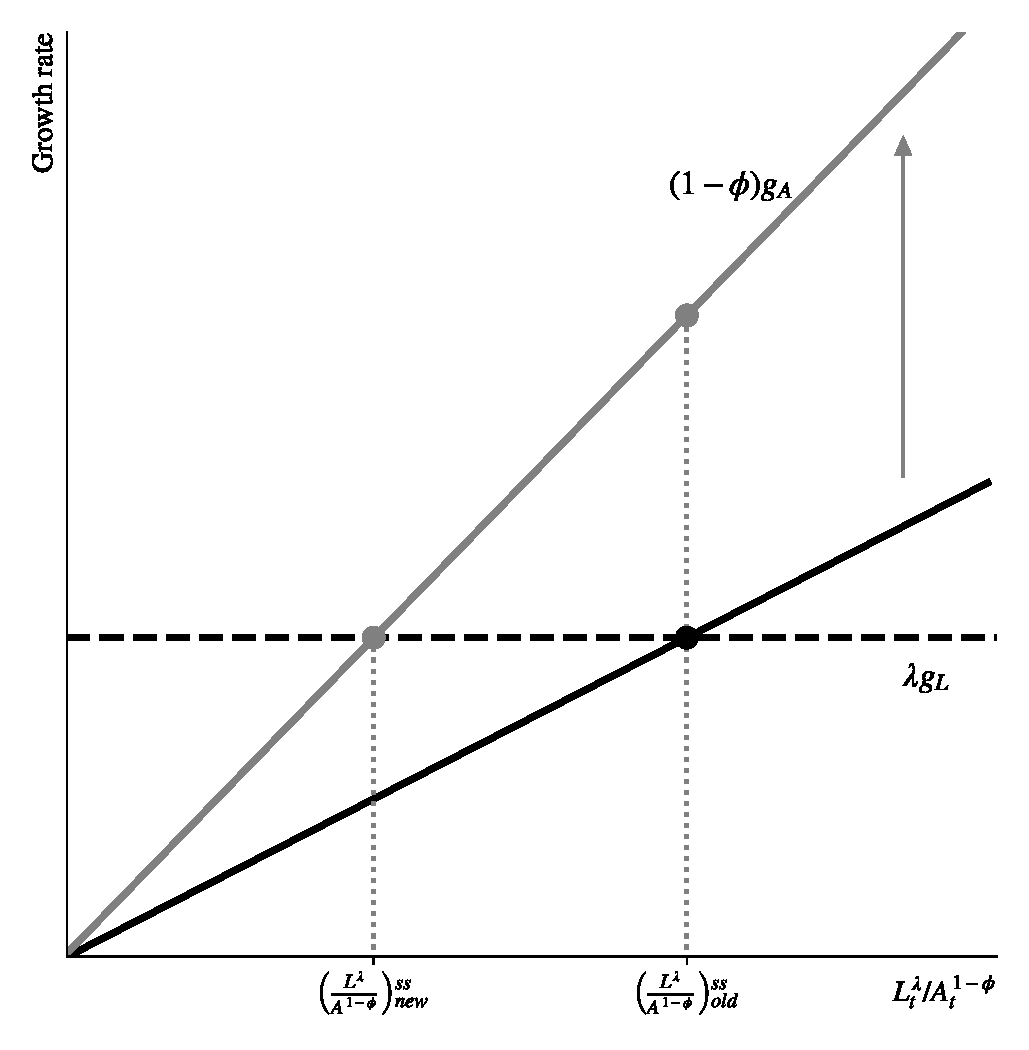
\includegraphics[height = 3in]{../Figures/fig-ch5-fig2.eps}
\end{center}
\end{frame}

\begin{frame}{Dynamics of $g_A$}
The Growth Rate of Productivity over Time
\begin{center}
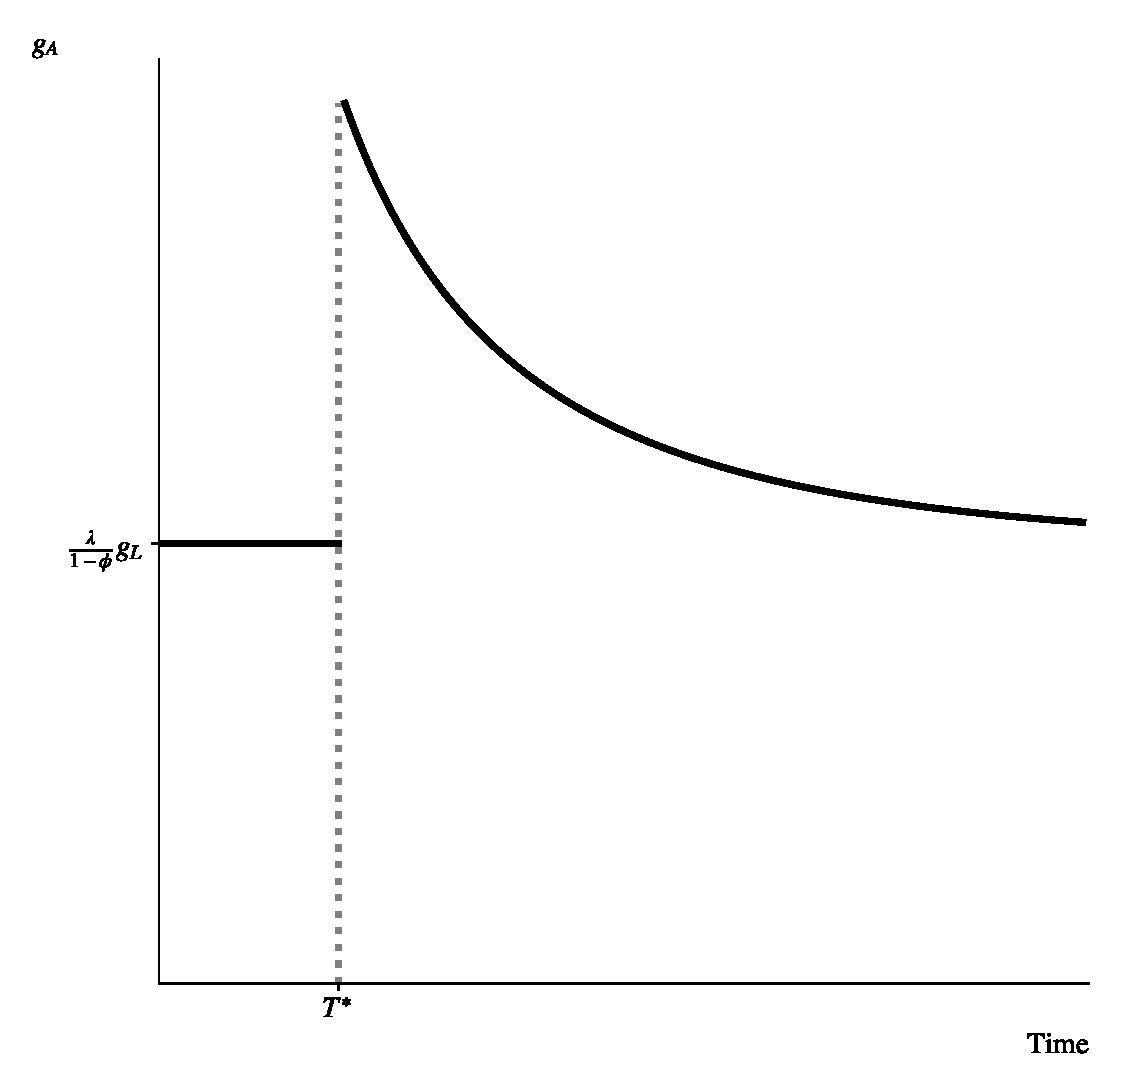
\includegraphics[height = 3in]{../Figures/fig-ch5-fig3.eps}
\end{center}
\end{frame}

\begin{frame}{Level effects}
The Level of Productivity over Time
\begin{center}
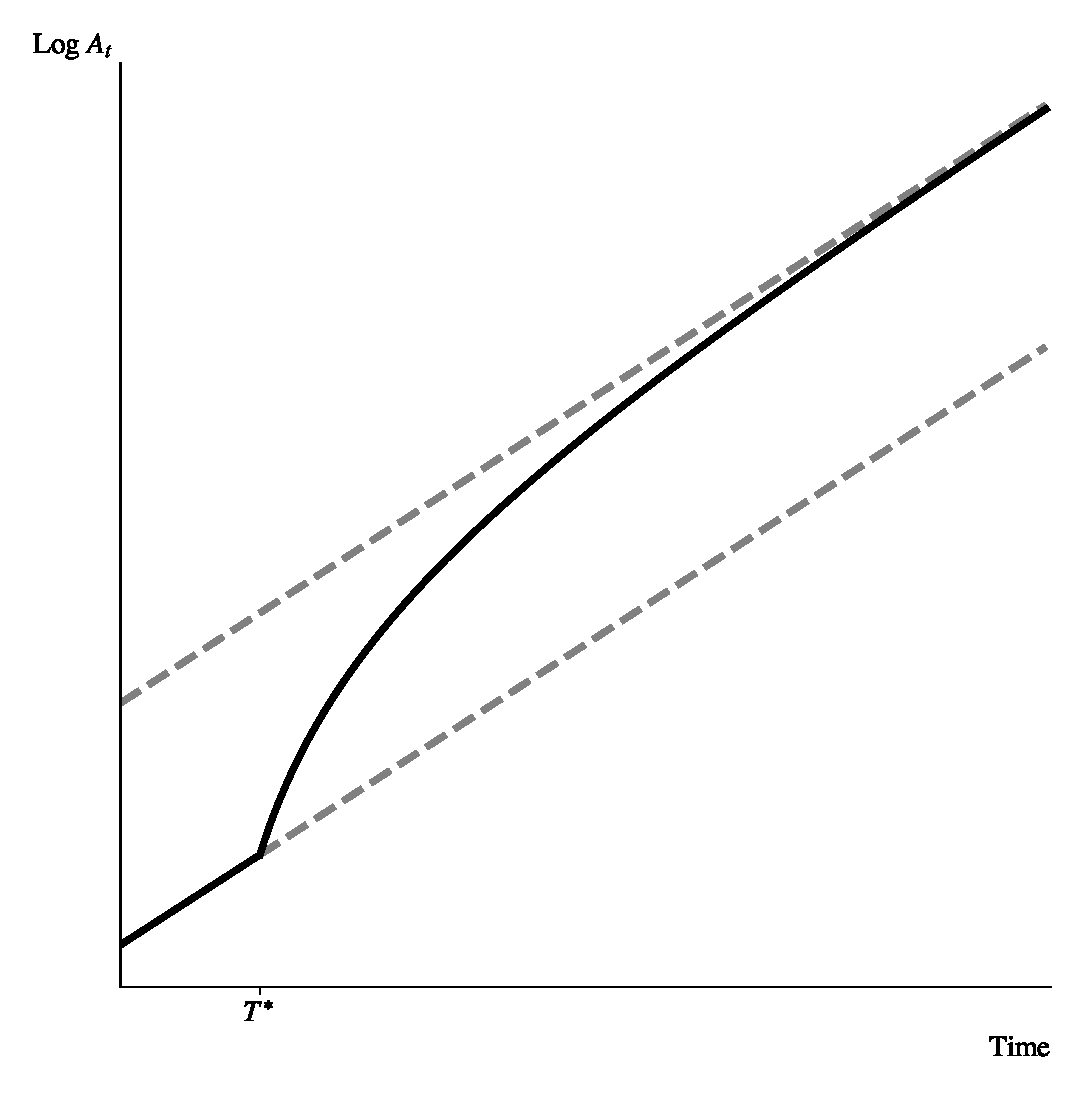
\includegraphics[height = 3in]{../Figures/fig-ch5-fig4.eps}
\end{center}
\end{frame}

\begin{frame}{The level of productivity}
$s_R$ influences the level of $A$. Make this explicit. We know in steady state:
\begin{equation}
	g_A^{ss} = \theta s_R \frac{L_t^{\lambda}}{A_t^{1-\phi}},
\end{equation}
and we can turn this around into a level of prod along a BGP
\begin{equation}
	A_t^{BGP} = \left(\frac{\theta s_R L_t^{\lambda}}{g_A^{ss}}\right)^{\frac{1}{1-\phi}}
\end{equation}
in log terms this is
\begin{equation}
	\ln A_t^{BGP} = \frac{1}{1-\phi}\frac{\theta s_R^{\lambda}}{g_A^{ss}} + \frac{\lambda}{1-\phi} \ln L_0 + \frac{\lambda}{1-\phi} g_L t
\end{equation}
The level of $A$ depends on the initial size of the economy, determined by $L_0$.
\end{frame}

\begin{frame}{The level of GDP per capita}
Recall that the level of GDP per capita is
\begin{equation}
	y_t^{BGP} = \left(\frac{s_I}{g_A + g_L + \delta}\right)^{\frac{\alpha}{1-\alpha}} (1-s_R) A_t 
\end{equation}
which depends on $A_t$ \textit{and} $(1-s_R)$. If you use $A_t^{BGP}$ for this it gets messy but
\begin{eqnarray*}
	\ln y_t^{BGP} &=& \frac{\alpha}{1-\alpha} \log \left(\frac{s_I}{g_A + g_L + \delta} \right) + \ln (1-s_R) \\ \nonumber
	&+& \frac{1}{1-\phi}\frac{\theta s_R^{\lambda}}{g_A^{ss}} + \frac{\lambda}{1-\phi} \ln L_0 + \frac{\lambda}{1-\phi} g_L t \nonumber
\end{eqnarray*}
and GDP per capita depends on initial market size, $L_0$. 
\end{frame}

\begin{frame}{The role of $s_R$}
Looking back at the level of GDP per capita, see two effects of $s_R$
\begin{itemize}
	\item If $s_R$ goes up, that raises productivity, and hence GDP per capita
	\item If $s_R$ goes up, that \textit{lowers} workers engaged in production, lowering GDP per capita
	\item There is an intermediate value of $s_R$ that maximizes GDP per capita
	\item It isn't true that $s_R = 1$ (all R\&D all the time) is best
	\item Return to this in Chapter 6
\end{itemize}
\end{frame}

\section{R\&D Decision}
\begin{frame}{The choice of R\&D}
All the long-run results hold regardless of the choice of $s_R$. But $s_R$ determines the level of productivity and GDP per capita. What determines $s_R$?
\begin{itemize}
	\item How do firms make the decision to do R\&D? Fixed cost versus flow of profits
	\item What determines the fixed cost? 
	\item What determines the flow of profits?
\end{itemize}
This requires an explicit description of an imperfect market which allows market power and profits. 
\end{frame}

\begin{frame}{The cost of R\&D}
For a potential firm, the fixed cost of finding a new idea to implement is
\begin{equation}
	F_t = w_t \frac{L_{Rt}}{dA},
\end{equation}
\begin{itemize}
	\item $w_t$ is the wage they have to pay to people to do R\&D
	\item $L_{Rt}/dA$ is how many workers it takes \textit{per idea}
	\item Potential firms take this ratio as given, determined in the aggregate
	\item Hence $F$ is wages/worker times worker/idea = wages/idea
\end{itemize}
\end{frame}

\begin{frame}{The benefit of R\&D}
For a potential firm, if they do have an idea they can earn some flow of profits each period. They care about the present discounted value of those profits, $V$, and will compare that to $F$.
\begin{equation}
	V_0 = \pi_0 + \frac{\pi_0(1+g_{\pi})}{1+r} + \frac{\pi_0(1+g_{\pi})^2}{(1+r)^2} + \frac{\pi_0(1+g_{\pi})^3}{(1+r)^3}+ ... \nonumber
\end{equation}
where $\pi_0$ is profits today, $r$ is the rate of return, and the growth rate of profits, $g_{\pi}$.
\begin{equation}
	V_0 = \pi_0 \sum_{t=0}^{\infty} \left(\frac{1+g_{\pi}}{1+r}\right)^{t}. \nonumber
\end{equation}
which solves to
\begin{equation}
	V_0 = \frac{\pi_0}{r-g_{\pi}}. \label{EQ_V} 
\end{equation}
\end{frame}

\begin{frame}{The benefit of R\&D}
Given this valuation
\begin{equation}
	V_0 = \frac{\pi_0}{r-g_{\pi}}. \label{EQ_V} 
\end{equation}
An idea is more valuable:
\begin{itemize}
	\item If initial profits are large - link this to market power
	\item If $r$ is low. $r$ is discount rate on the future and/or return on alternative assets.
	\item $g_{\pi}$ is high - link this to growth of economy
\end{itemize}
\end{frame}

\begin{frame}{The innovators decisions}
We have lots of potential firms, and so long as $V_0 > F$ they will continue to do R\&D. Assume they enter until $V_0 = F$,
\begin{equation}
	\frac{\pi_t}{r-g_{\pi}} = w_t \frac{L_{Rt}}{dA}. \nonumber
\end{equation}
Ultimately we want to solve this for $s_R$, which recall is $L_{Rt} = s_R L_t$, so really we are solving for $L_{Rt}$. But we need
\begin{itemize}
	\item Initial profits
	\item Growth rate of profits
	\item Wage
\end{itemize}
\end{frame}

\section{Market Structure}
\begin{frame}{Overview}
The overall structure of this economy is more complex than Solow. An overview:
\begin{itemize}
	\item At the ``top'' there are a set of final goods firms (e.g. Target). They stock intermediate goods that consumers purchase (e.g. Diet Coke, toothbrushes, t-shirts). 
	\item Final good firms are competitive (no profits) and there is no innovation here. They stock goods only. 
	\item Final good firms like to stock a variety of goods
	\item Intermediate good firms supply the individual goods to final good firms (e.g. Coca-Cola, Oral-B, Hanes)
	\item Intermediate firms are monopolists (e.g. only Coca-Cola can sell Coke) and earn profits
	\item A new idea represents a new variety of intermediate good which can earn those profits
\end{itemize}
\end{frame}

\begin{frame}{Final good firms}
The final good firms produce GDP using
\begin{equation}
	Y = L_{Y}^{1-\alpha} \sum_{j=1}^{A} x_{j}^{\alpha}. \nonumber
\end{equation}
\begin{itemize}
	\item $L_Y$ are production workers (not R\&D workers)
	\item $x_j$ is the amount of each product they stock
	\item $A$ is the \textit{number} of products they stock
	\item $\alpha$ captures how much they like variety.
\end{itemize}
Note that this $Y$ is GDP because intermediate good sales to the final good firm are explicitly not accounted for in GDP. 
\end{frame}

\begin{frame}{Final good maximization}
We assume final good firms maximize profits. They are competitive so profits end up at zero, but they still try. To do this they set marginal product equal marginal cost. For labor:
\begin{equation}
	w = (1-\alpha) \frac{Y}{L_Y}, \label{EQ_final_w}
\end{equation}
and for an individual product $j$
\begin{equation}
	p_j = \alpha L_Y^{1-\alpha} x_j^{\alpha-1}. \label{EQ_final_pj}
\end{equation}
this is the equation of a demand curve for product $j$. The higher $p_j$, the lower demand.
\end{frame}

\begin{frame}{Intermediate good firms}
Each intermediate firm produces their good using the function $x_j = K_j$, using only capital, which costs $r$ per unit of capital. Their profits are:
\begin{equation}
	\pi_j = p_j x_j - r x_j. \nonumber
\end{equation}
They are a monopolist, so they know how $p_j$ responds to their choice of $x_j$. That is, they know what the demand curve of final good firms looks like. They set marginal revenue equal to marginal cost
\begin{equation}
	p + \frac{\partial p}{\partial x}x = r. \nonumber
\end{equation}
\end{frame}

\begin{frame}{Intermediate good firms}
Take the MR = MC condition
\begin{equation}
	p + \frac{\partial p}{\partial x}x = r. \nonumber
\end{equation}
divide by $p$
\begin{equation}
	1 + \frac{\partial p}{\partial x}\frac{x}{p} = \frac{r}{p}. \nonumber
\end{equation}
and the ratio on the left is the elasticity of price with respect to quantity, which from final goods firms is equal to $\alpha - 1$. So
\begin{equation}
	1 + (\alpha-1) = \frac{r}{p} \nonumber
\end{equation}
and 
\begin{equation}
	p = \frac{1}{\alpha}r. \label{EQ_markup}
\end{equation}
\end{frame}

\begin{frame}{Intermediate good firms}
Given the pricing result
\begin{equation}
	p = \frac{1}{\alpha}r \label{EQ_markup}
\end{equation}
this represents a \textit{markup} of the price over the marginal cost. If $\alpha$ goes to one, the final good firm doesn't care about variety, and the markup is lower (and vice versa). 

\vspace{.25in}\noindent This market power is what will drive profits and make innovation to create a new intermediate good worth it. This matches the intuition from Chapter 4 that innovation depends on charging a price higher than marginal cost.
\end{frame}

\section{Aggregate outcomes}
\begin{frame}{Adding up}
Given the ``micro'' results on final good firms and intermediate firms.
\begin{itemize}
	\item Each intermediate firm has an identical technology, so $p_j = r/\alpha$ for all
	\item Because they are identical, they demand identical amounts of capital, $x_j = K/A$
\end{itemize}
so final good firms produce
\begin{equation}
	Y = L_Y^{1-\alpha} A x^{\alpha}.
\end{equation}
which solves to
\begin{eqnarray}
	Y &=& L_Y^{1-\alpha} A \left(\frac{K}{A} \right)^{\alpha} \nonumber \\ 
	  &=& K^{\alpha} (AL_Y)^{1-\alpha}.
\end{eqnarray}
Despite the complexity, GDP has a similar function to the Solow
\end{frame}

\begin{frame}{Wages and profits}
Solve for things we need to know. Start with the wage. Given the first order condition from final good firms:
\begin{equation}
	w_t L_{Yt} = (1-\alpha)Y_t, \nonumber
\end{equation}
$(1-\alpha)$ of GDP gets spent on workers. The other $\alpha$ must get spent on intermediate goods (final good firms don't have profits). The revenues of any given intermediate firm are thus
\begin{equation}
	p_j x_j = \frac{\alpha Y_t}{A_t}
\end{equation}
or the $A$ firms split the $\alpha Y_t$ in total profits
\end{frame}

\begin{frame}{Profits per firm}
What are profits for a firm?
\begin{eqnarray}
	\pi_t &=& p_t x_t - r_t x_t \nonumber \\
	      &=& (p_t - \alpha p_t) x_t \nonumber \\
	      &=& (1-\alpha) p_t x_t, \nonumber
\end{eqnarray}
and plug in for firm revenues $p_j x_j = \frac{\alpha Y_t}{A_t}$
\begin{equation}
	\pi_t = (1-\alpha) \alpha \frac{Y_t}{A_t}.\label{EQ_pi_j}
\end{equation}
are profits per intermediate firm. This is the initial profits that go into the valuation of an idea.
\end{frame}

\begin{frame}{Growth rate of profits}
How fast do profits grow? Profits are
\begin{equation}
	\pi_t = (1-\alpha) \alpha \frac{Y_t}{A_t}.\label{EQ_pi_j}
\end{equation}
so profits grow at the rate (along a BGP) of
\begin{equation}
	g_{\pi} = g_Y - g_A. \nonumber
\end{equation}
but we know along a BGP that $g_Y = g_L + g_A$ so
\begin{equation}
	g_{\pi} = g_L
\end{equation}
or profits grow as fast as the market.
\end{frame}

\section{R\&D Solution}
\begin{frame}{Solving for $s_R$}
We have all the pieces to go back to this condition for innovation:
\begin{equation}
	\frac{\pi_t}{r-g_{\pi}} = w_t \frac{L_{Rt}}{dA}. \nonumber
\end{equation}
so 
\begin{equation}
	\frac{\alpha(1-\alpha) \frac{Y_t}{A_t}}{r-g_L} = (1-\alpha)\frac{Y_t}{L_{Yt}} \frac{L_{Rt}}{g_A A_t}. \nonumber
\end{equation}
which solves for
\begin{equation}
	\frac{s_R}{1-s_R} = \frac{\alpha(1-\alpha)}{(1-\alpha)}\frac{g_A}{r-g_L}. \label{EQ_sR_romer}
\end{equation}

\end{frame}

\begin{frame}{Solving for $s_R$}
Given the solution
\begin{equation}
	\frac{s_R}{1-s_R} = \frac{\alpha(1-\alpha)}{(1-\alpha)}\frac{g_A}{r-g_L}. \label{EQ_sR_romer}
\end{equation}
$s_R$ is higher:
\begin{itemize}
	\item If $g_A$ is higher. If innovations come quickly, it pays to hire R\&D workers
	\item If $r$ is lower. If the future matters more, it pays to do R\&D
	\item If $g_L$ is higher. If the market will grow quickly, it pays to do R\&D
	\item If $\alpha(1-\alpha)$ (profits as a share of GDP) is higher
	\item If $(1-\alpha)$ (wages as a share of GDP) is lower
\end{itemize}
\end{frame}

\end{document}